\documentclass[]{report}
\usepackage{lmodern}
\usepackage{amssymb,amsmath}
\usepackage{ifxetex,ifluatex}
\usepackage{fixltx2e} % provides \textsubscript
\ifnum 0\ifxetex 1\fi\ifluatex 1\fi=0 % if pdftex
  \usepackage[T1]{fontenc}
  \usepackage[utf8]{inputenc}
\else % if luatex or xelatex
  \ifxetex
    \usepackage{mathspec}
  \else
    \usepackage{fontspec}
  \fi
  \defaultfontfeatures{Ligatures=TeX,Scale=MatchLowercase}
\fi
% use upquote if available, for straight quotes in verbatim environments
\IfFileExists{upquote.sty}{\usepackage{upquote}}{}
% use microtype if available
\IfFileExists{microtype.sty}{%
\usepackage{microtype}
\UseMicrotypeSet[protrusion]{basicmath} % disable protrusion for tt fonts
}{}
\usepackage{hyperref}
\hypersetup{unicode=true,
            pdftitle={Data 624 - Group 2 Homework Part 2},
            pdfauthor={Vinicio Haro; Sang Yoon (Andy) Hwang; Julian McEachern; Jeremy O'Brien; Bethany Poulin},
            pdfborder={0 0 0},
            breaklinks=true}
\urlstyle{same}  % don't use monospace font for urls
\usepackage{color}
\usepackage{fancyvrb}
\newcommand{\VerbBar}{|}
\newcommand{\VERB}{\Verb[commandchars=\\\{\}]}
\DefineVerbatimEnvironment{Highlighting}{Verbatim}{commandchars=\\\{\}}
% Add ',fontsize=\small' for more characters per line
\usepackage{framed}
\definecolor{shadecolor}{RGB}{248,248,248}
\newenvironment{Shaded}{\begin{snugshade}}{\end{snugshade}}
\newcommand{\AlertTok}[1]{\textcolor[rgb]{0.94,0.16,0.16}{#1}}
\newcommand{\AnnotationTok}[1]{\textcolor[rgb]{0.56,0.35,0.01}{\textbf{\textit{#1}}}}
\newcommand{\AttributeTok}[1]{\textcolor[rgb]{0.77,0.63,0.00}{#1}}
\newcommand{\BaseNTok}[1]{\textcolor[rgb]{0.00,0.00,0.81}{#1}}
\newcommand{\BuiltInTok}[1]{#1}
\newcommand{\CharTok}[1]{\textcolor[rgb]{0.31,0.60,0.02}{#1}}
\newcommand{\CommentTok}[1]{\textcolor[rgb]{0.56,0.35,0.01}{\textit{#1}}}
\newcommand{\CommentVarTok}[1]{\textcolor[rgb]{0.56,0.35,0.01}{\textbf{\textit{#1}}}}
\newcommand{\ConstantTok}[1]{\textcolor[rgb]{0.00,0.00,0.00}{#1}}
\newcommand{\ControlFlowTok}[1]{\textcolor[rgb]{0.13,0.29,0.53}{\textbf{#1}}}
\newcommand{\DataTypeTok}[1]{\textcolor[rgb]{0.13,0.29,0.53}{#1}}
\newcommand{\DecValTok}[1]{\textcolor[rgb]{0.00,0.00,0.81}{#1}}
\newcommand{\DocumentationTok}[1]{\textcolor[rgb]{0.56,0.35,0.01}{\textbf{\textit{#1}}}}
\newcommand{\ErrorTok}[1]{\textcolor[rgb]{0.64,0.00,0.00}{\textbf{#1}}}
\newcommand{\ExtensionTok}[1]{#1}
\newcommand{\FloatTok}[1]{\textcolor[rgb]{0.00,0.00,0.81}{#1}}
\newcommand{\FunctionTok}[1]{\textcolor[rgb]{0.00,0.00,0.00}{#1}}
\newcommand{\ImportTok}[1]{#1}
\newcommand{\InformationTok}[1]{\textcolor[rgb]{0.56,0.35,0.01}{\textbf{\textit{#1}}}}
\newcommand{\KeywordTok}[1]{\textcolor[rgb]{0.13,0.29,0.53}{\textbf{#1}}}
\newcommand{\NormalTok}[1]{#1}
\newcommand{\OperatorTok}[1]{\textcolor[rgb]{0.81,0.36,0.00}{\textbf{#1}}}
\newcommand{\OtherTok}[1]{\textcolor[rgb]{0.56,0.35,0.01}{#1}}
\newcommand{\PreprocessorTok}[1]{\textcolor[rgb]{0.56,0.35,0.01}{\textit{#1}}}
\newcommand{\RegionMarkerTok}[1]{#1}
\newcommand{\SpecialCharTok}[1]{\textcolor[rgb]{0.00,0.00,0.00}{#1}}
\newcommand{\SpecialStringTok}[1]{\textcolor[rgb]{0.31,0.60,0.02}{#1}}
\newcommand{\StringTok}[1]{\textcolor[rgb]{0.31,0.60,0.02}{#1}}
\newcommand{\VariableTok}[1]{\textcolor[rgb]{0.00,0.00,0.00}{#1}}
\newcommand{\VerbatimStringTok}[1]{\textcolor[rgb]{0.31,0.60,0.02}{#1}}
\newcommand{\WarningTok}[1]{\textcolor[rgb]{0.56,0.35,0.01}{\textbf{\textit{#1}}}}
\usepackage{graphicx,grffile}
\makeatletter
\def\maxwidth{\ifdim\Gin@nat@width>\linewidth\linewidth\else\Gin@nat@width\fi}
\def\maxheight{\ifdim\Gin@nat@height>\textheight\textheight\else\Gin@nat@height\fi}
\makeatother
% Scale images if necessary, so that they will not overflow the page
% margins by default, and it is still possible to overwrite the defaults
% using explicit options in \includegraphics[width, height, ...]{}
\setkeys{Gin}{width=\maxwidth,height=\maxheight,keepaspectratio}
\IfFileExists{parskip.sty}{%
\usepackage{parskip}
}{% else
\setlength{\parindent}{0pt}
\setlength{\parskip}{6pt plus 2pt minus 1pt}
}
\setlength{\emergencystretch}{3em}  % prevent overfull lines
\providecommand{\tightlist}{%
  \setlength{\itemsep}{0pt}\setlength{\parskip}{0pt}}
\setcounter{secnumdepth}{0}

%%% Use protect on footnotes to avoid problems with footnotes in titles
\let\rmarkdownfootnote\footnote%
\def\footnote{\protect\rmarkdownfootnote}

%%% Change title format to be more compact
\usepackage{titling}

% Create subtitle command for use in maketitle
\providecommand{\subtitle}[1]{
  \posttitle{
    \begin{center}\large#1\end{center}
    }
}

\setlength{\droptitle}{-2em}

  \title{Data 624 - Group 2\\
Homework Part 2}
    \pretitle{\vspace{\droptitle}\centering\huge}
  \posttitle{\par}
    \author{Vinicio Haro \\ Sang Yoon (Andy) Hwang \\ Julian McEachern \\ Jeremy O'Brien \\ Bethany Poulin}
    \preauthor{\centering\large\emph}
  \postauthor{\par}
      \predate{\centering\large\emph}
  \postdate{\par}
    \date{16 December 2019}

% set plain style for page numbers
\pagestyle{plain}
\raggedbottom

% change font
\usepackage{fontspec}
\setmainfont{Arial}

% create color block quotes
\usepackage[dvipsnames]{xcolor}
\usepackage{tcolorbox}     
\newtcolorbox{question}[1]{colback=white, colframe=Emerald ,fonttitle=\bfseries, title=#1}

\newtcolorbox{subquestion}[1]{colback=white,colframe=white, coltitle=Emerald!75!black, detach title, before upper={\tcbtitle\quad\hangindent7mm}, title={#1},fonttitle=\bfseries, fontupper=\bfseries}

% remove "chapter" from chapter title
\usepackage{titlesec}

\titleformat{\chapter}
  {\normalfont\LARGE\bfseries}{\thechapter}{1em}{}
\titlespacing*{\chapter}{0pt}{3.5ex plus 1ex minus .2ex}{2.3ex plus .2ex}

\usepackage{titling}
\pretitle{\begin{flushright}\LARGE}
\posttitle{\par\end{flushright}\vskip 0.5em}
\preauthor{\begin{flushright}\large \lineskip 0.5em}
\postauthor{\par\end{flushright}}
\predate{\begin{flushright}\large}
\postdate{\par\end{flushright}}


% wrap text
\usepackage{geometry}[textwidth=6in]

% kable 
\usepackage{tabu}
\usepackage{float} 

% multicolumn
\usepackage{multicol}
\usepackage{booktabs}
\usepackage{longtable}
\usepackage{array}
\usepackage{multirow}
\usepackage{wrapfig}
\usepackage{float}
\usepackage{colortbl}
\usepackage{pdflscape}
\usepackage{tabu}
\usepackage{threeparttable}
\usepackage{threeparttablex}
\usepackage[normalem]{ulem}
\usepackage{makecell}
\usepackage{xcolor}

\begin{document}
\maketitle

{
\setcounter{tocdepth}{2}
\tableofcontents
}
\hypertarget{Overview}{%
\chapter*{Getting Started}\label{Overview}}
\addcontentsline{toc}{chapter}{Getting Started}

\hypertarget{overview}{%
\section{Overview}\label{overview}}

Include details on our process in creating this document.

\hypertarget{dependencies}{%
\section{Dependencies}\label{dependencies}}

\begin{Shaded}
\begin{Highlighting}[]
\CommentTok{# Predicitve Modeling}
\KeywordTok{libraries}\NormalTok{(}\StringTok{"AppliedPredictiveModeling"}\NormalTok{, }\StringTok{"mice"}\NormalTok{, }\StringTok{"caret"}\NormalTok{, }\StringTok{"tidyverse"}\NormalTok{, }
    \StringTok{"impute"}\NormalTok{, }\StringTok{"pls"}\NormalTok{, }\StringTok{"caTools"}\NormalTok{, }\StringTok{"mlbench"}\NormalTok{)}
\CommentTok{# Formatting Libraries}
\KeywordTok{libraries}\NormalTok{(}\StringTok{"default"}\NormalTok{, }\StringTok{"knitr"}\NormalTok{, }\StringTok{"kableExtra"}\NormalTok{)}
\CommentTok{# Plotting Libraries}
\KeywordTok{libraries}\NormalTok{(}\StringTok{"ggplot2"}\NormalTok{, }\StringTok{"grid"}\NormalTok{, }\StringTok{"ggfortify"}\NormalTok{)}
\end{Highlighting}
\end{Shaded}

\newpage

\hypertarget{AS-1}{%
\chapter*{Assignment 1}\label{AS-1}}
\addcontentsline{toc}{chapter}{Assignment 1}

\addcontentsline{toc}{subsection}{Kuhn and Johnson 6.3}

\begin{question}{Kuhn and Johnson 6.3}A chemical manufacturing process for a pharmaceutical product was discussed in Sect.1.4. In this problem, the objective is to understand the relationship between biological measurements of the raw materials (predictors), measurements of the manufacturing process (predictors), and the response of product yield. Biological predictors cannot be changed but can be used to assess the quality of the raw material before processing. On the other hand, manufacturing process predictors can be changed in the manufacturing process. Improving product yield by 1\% will boost revenue by approximately one hundred thousand dollars per batch:\end{question}

\begin{subquestion}{(a).}Start R and use these commands to load the data:
\end{subquestion}

The matrix processPredictors contains the 57 predictors (12 describing
the input biological material and 45 describing the process predictors)
for the 176 manufacturing runs. yield contains the percent yield for
each run.

\begin{Shaded}
\begin{Highlighting}[]
\KeywordTok{data}\NormalTok{(}\StringTok{"ChemicalManufacturingProcess"}\NormalTok{)}
\end{Highlighting}
\end{Shaded}

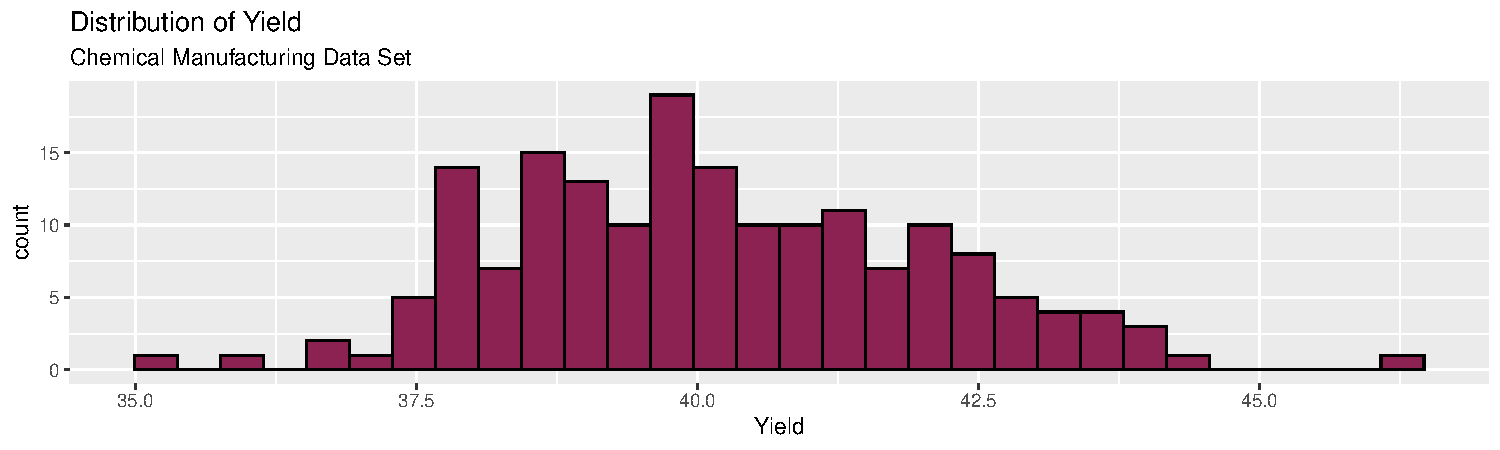
\includegraphics{Homework-Two_files/figure-latex/unnamed-chunk-2-1.pdf}

\begin{subquestion}{(b).} A small percentage of cells in the predictor set contain missing values. Use an imputation function to fill in these missing values (e.g., see Sect. 3.8). 
\end{subquestion}

ManufacturingProcess03 has the largest volume of missing data followed
by ManufacturingProcess11. Given that each variable has less than 25\%
of data missing, we should introduce methods of imputation. For our
purposes, we will use the MICE method. MICE is formally known as
Multiple Imputation with Chained Equations. On a high level, MICE is
built off a tehcnique known as the Gibbs sampler. The Gibbs sampler is a
Markov chain based on Monte Carlo. MICE iterates drawing estimates of
missing values and parameters related to the distribution of said
variables. Chained equations are generally faster than the monte carlo
based Gibbs sampler. MICE has 5 imputations listed as its default.
predictive mean matching is also a default method for MICE. PMM does a
better job at keeping non-linear relationships within individual
variables.

In addition to MICE, we drop variables that have near zero variance,
however we point out that only one variable was dropped. We still
include it as a process step to follow the literature's specifications.
After completing MICE, we no longer had missing data in our set. We
examined other imputation methods such as KNN but determined that there
was no significant change in the summary statistics across different
imputation methods.

\begin{table}[H]

\caption{\label{tab:kj-6.3b}Distribution of Missing data in Chemical Manufacturing Process}
\centering
\begin{tabular}{l|r|l|r}
\hline
Variable & Count & Variable & Count\\
\hline
\rowcolor{gray!6}  ManufacturingProcess03 & 15 & BiologicalMaterial01 & 0\\
\hline
ManufacturingProcess11 & 10 & BiologicalMaterial02 & 0\\
\hline
\rowcolor{gray!6}  ManufacturingProcess10 & 9 & BiologicalMaterial03 & 0\\
\hline
ManufacturingProcess25 & 5 & BiologicalMaterial04 & 0\\
\hline
\rowcolor{gray!6}  ManufacturingProcess26 & 5 & BiologicalMaterial05 & 0\\
\hline
ManufacturingProcess27 & 5 & BiologicalMaterial06 & 0\\
\hline
\rowcolor{gray!6}  ManufacturingProcess28 & 5 & BiologicalMaterial07 & 0\\
\hline
ManufacturingProcess29 & 5 & BiologicalMaterial08 & 0\\
\hline
\rowcolor{gray!6}  ManufacturingProcess30 & 5 & BiologicalMaterial09 & 0\\
\hline
ManufacturingProcess31 & 5 & BiologicalMaterial10 & 0\\
\hline
\rowcolor{gray!6}  ManufacturingProcess33 & 5 & BiologicalMaterial11 & 0\\
\hline
ManufacturingProcess34 & 5 & BiologicalMaterial12 & 0\\
\hline
\rowcolor{gray!6}  ManufacturingProcess35 & 5 & ManufacturingProcess09 & 0\\
\hline
ManufacturingProcess36 & 5 & ManufacturingProcess13 & 0\\
\hline
\rowcolor{gray!6}  ManufacturingProcess02 & 3 & ManufacturingProcess15 & 0\\
\hline
ManufacturingProcess06 & 2 & ManufacturingProcess16 & 0\\
\hline
\rowcolor{gray!6}  ManufacturingProcess01 & 1 & ManufacturingProcess17 & 0\\
\hline
ManufacturingProcess04 & 1 & ManufacturingProcess18 & 0\\
\hline
\rowcolor{gray!6}  ManufacturingProcess05 & 1 & ManufacturingProcess19 & 0\\
\hline
ManufacturingProcess07 & 1 & ManufacturingProcess20 & 0\\
\hline
\rowcolor{gray!6}  ManufacturingProcess08 & 1 & ManufacturingProcess21 & 0\\
\hline
ManufacturingProcess12 & 1 & ManufacturingProcess32 & 0\\
\hline
\rowcolor{gray!6}  ManufacturingProcess14 & 1 & ManufacturingProcess37 & 0\\
\hline
ManufacturingProcess22 & 1 & ManufacturingProcess38 & 0\\
\hline
\rowcolor{gray!6}  ManufacturingProcess23 & 1 & ManufacturingProcess39 & 0\\
\hline
ManufacturingProcess24 & 1 & ManufacturingProcess42 & 0\\
\hline
\rowcolor{gray!6}  ManufacturingProcess40 & 1 & ManufacturingProcess43 & 0\\
\hline
ManufacturingProcess41 & 1 & ManufacturingProcess44 & 0\\
\hline
\end{tabular}
\end{table}

\begin{subquestion}{(c).} Split the data into a training and a test set, pre-process the data, and tune a model of your choice from this chapter. What is the optimal value of the performance metric? 
\end{subquestion}

We will build a PLS model also known as partial least squares. PLS is a
statistical method that fits a linear regression model by projecting the
feature variables and response variable to some new space via a mapping
function. Because of this projection mechanisim, for both predictors and
the response, the method becomes bilinear or simply known as linear with
respect to to each of the variable types. PLS also has certain
advantages over other methods such as being more robust to dealing with
issues arising from multicolinearity.

For our PLS model, we partitioned the data by taking 80\% of the data as
training and the remaining 20\% as testing subsets. We also apply center
and scaling arguments set to true. We built a standard PLS model and
evaluated the root mean summary areas to determine the optimal number of
components to select. In our case, 41 components seemed to cause the
root meean summary area to flatten. Any changes after 41 were marginal.
We generate performance metrics agasint the training data for our
baseline PLS model with all components.

\begin{table}[H]

\caption{\label{tab:kj-6.3c}PLS Performance Metrics on Training Subset}
\centering
\begin{tabular}{l|r}
\hline
  & x\\
\hline
\rowcolor{gray!6}  RMSE & 1.3067750\\
\hline
Rsquared & 0.4934303\\
\hline
\rowcolor{gray!6}  MAE & 1.0546925\\
\hline
\end{tabular}
\end{table}

Our Baseline PLS model generates a RMSE of 1.3. In addition, the model
captures 49\% of data variability. We include the visualizations
pertaining to the RMSEP values against Yield. At roughly 41 components,
the RMSEP flattens.

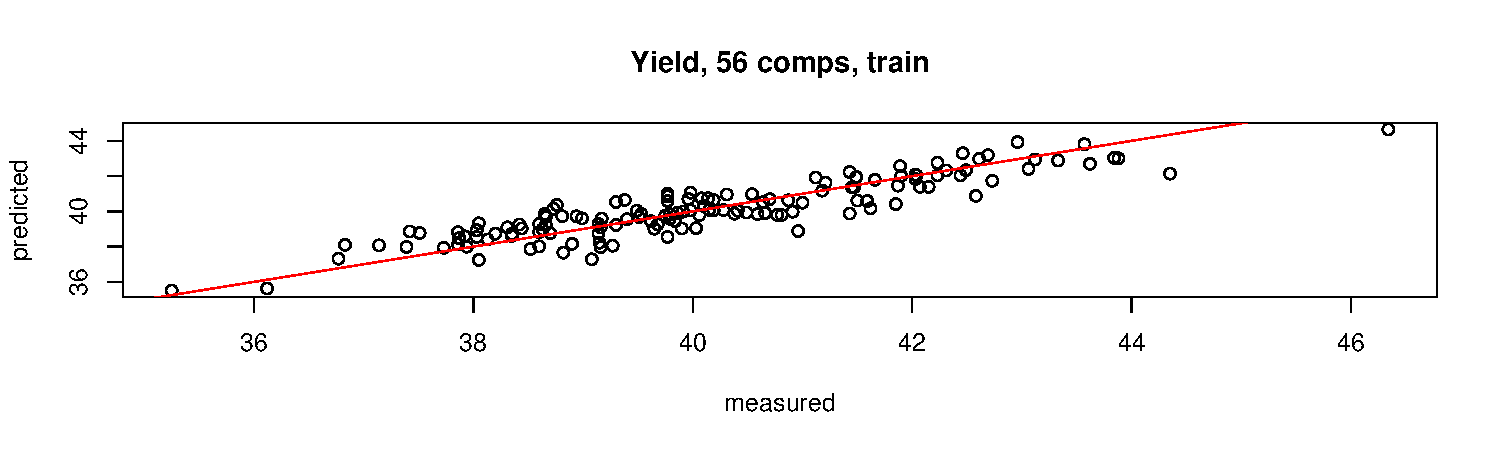
\includegraphics{Homework-Two_files/figure-latex/kj-6.3c2-1.pdf}
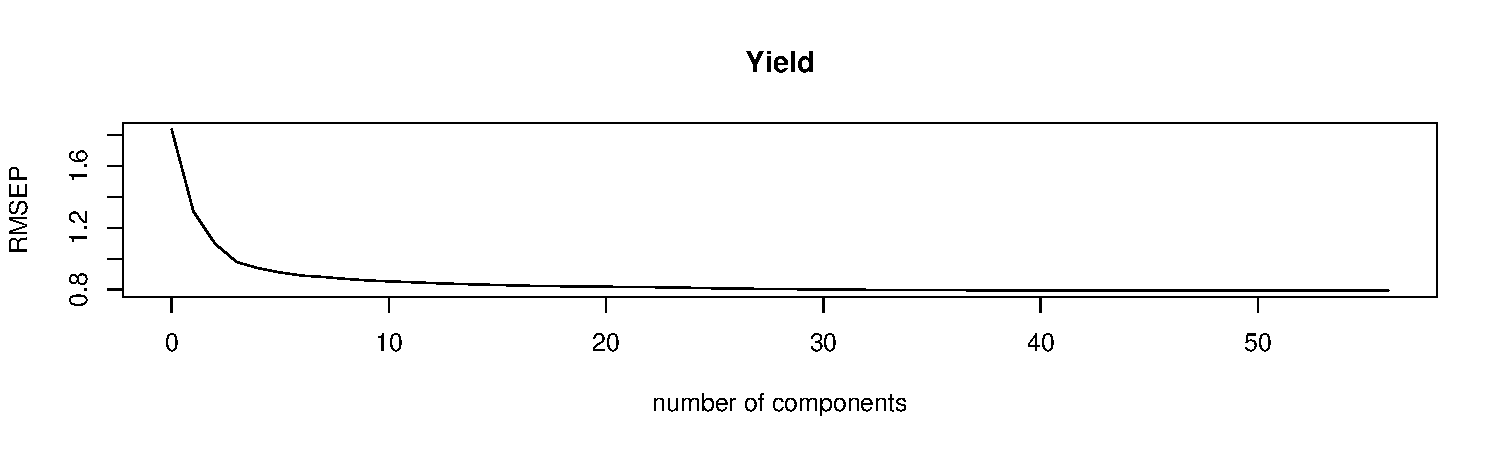
\includegraphics{Homework-Two_files/figure-latex/kj-6.3c2-2.pdf}

\begin{subquestion}{(d).} Predict the response for the test set. What is the value of the performance metric and how does this compare with the resampled performance metric on the training set? 
\end{subquestion}

\begin{table}[H]

\caption{\label{tab:kj-6.3d}PLS Performance Metrics on Test Subset}
\centering
\begin{tabular}{l|r}
\hline
  & x\\
\hline
\rowcolor{gray!6}  RMSE & 1.2586244\\
\hline
Rsquared & 0.5653015\\
\hline
\rowcolor{gray!6}  MAE & 0.9959796\\
\hline
\end{tabular}
\end{table}

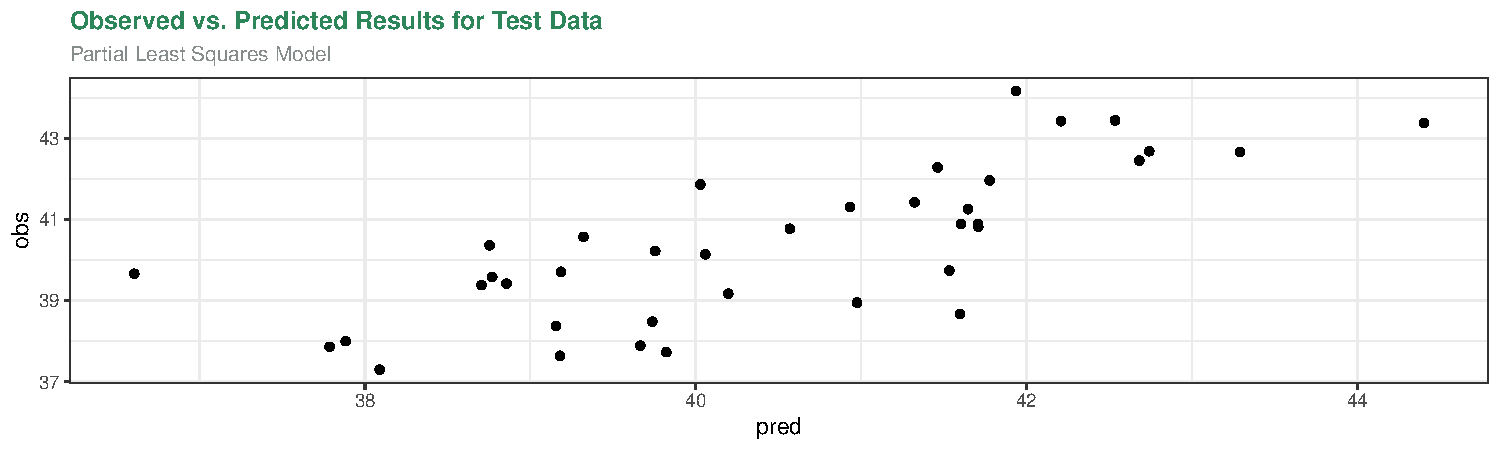
\includegraphics{Homework-Two_files/figure-latex/kj-6.3d-1.pdf}

We see an increased R squared against the test data with 56 percent of
the data variability accounted for. We also see the RMSE decrease to 1.2
from 1.3. There is also a slight decrease in the MAE. Overall, it seems
that using PLS with 41 components imporved the performance metrics vs
our baseline PLS model with all components.

\begin{subquestion}{(e).} Which predictors are most important in the model you have trained? Do either the biological or process predictors dominate the list? 
\end{subquestion}

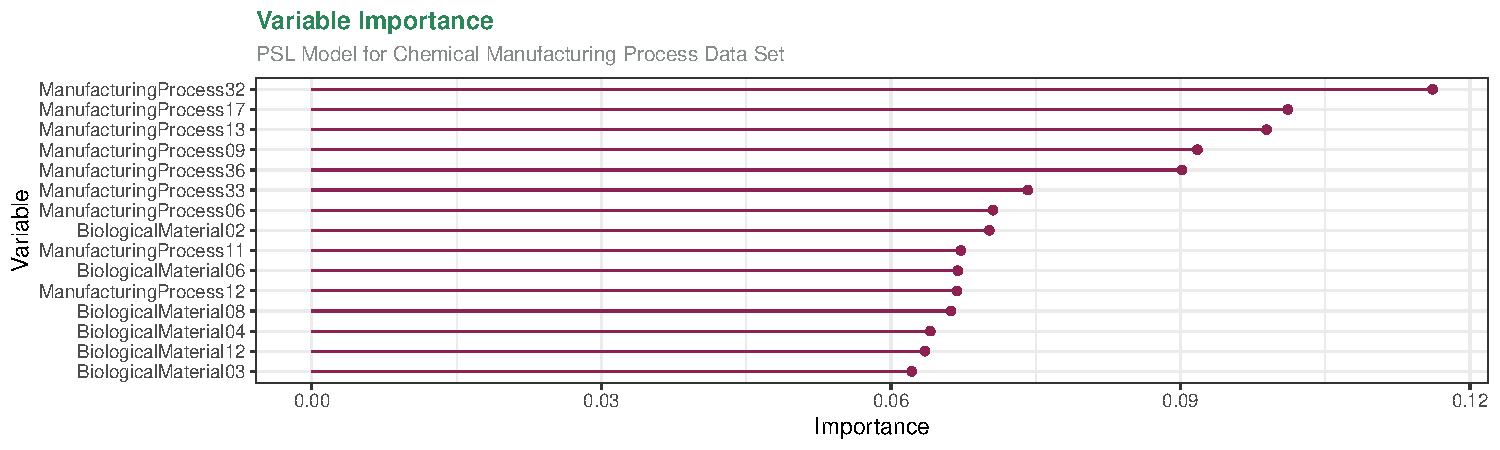
\includegraphics{Homework-Two_files/figure-latex/kj-6.3e-1.pdf}

VarImp allows us to identify the variables by name and compute their
importance. ManufacturingProcess32 was flagged as the most important
predictor overall and within the group of other Manufacturing Process
variables. BiologicalMaterial02 was the most important variable within
the BiologicalMaterial group but ranks 6th overall. The variable
importance rankings are dominated by Manufacturing Process 9 to 6 within
the top 15 predictors.

\begin{subquestion}{(f).} Explore the relationships between each of the top predictors and the response. How could this information be helpful in improving yield in future runs of the manufacturing process?
\end{subquestion}

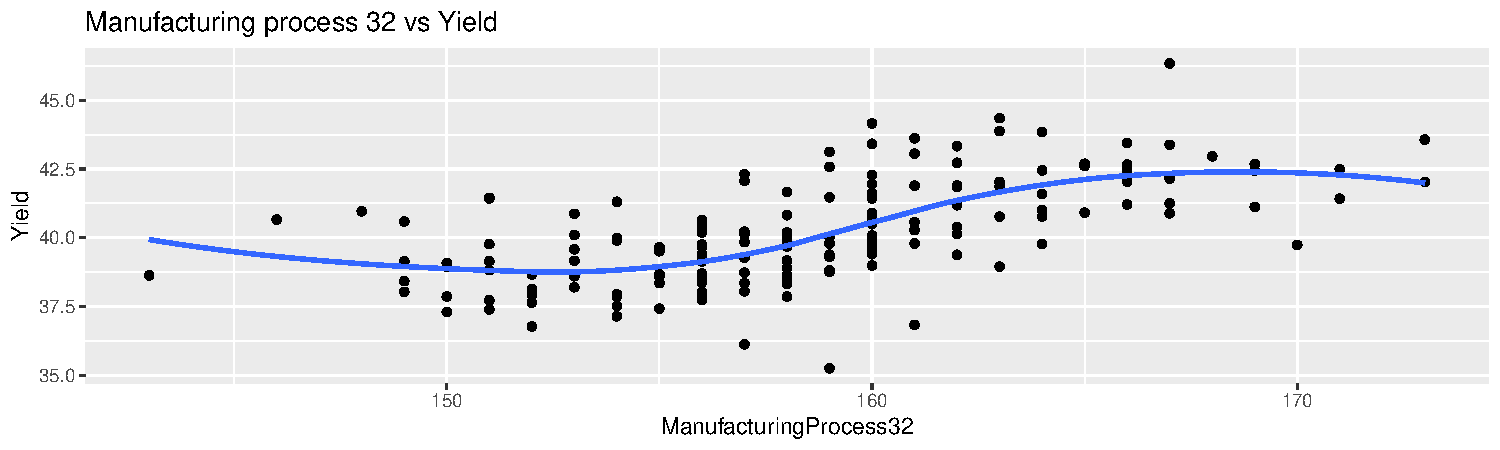
\includegraphics{Homework-Two_files/figure-latex/kj-6.3f-1.pdf}
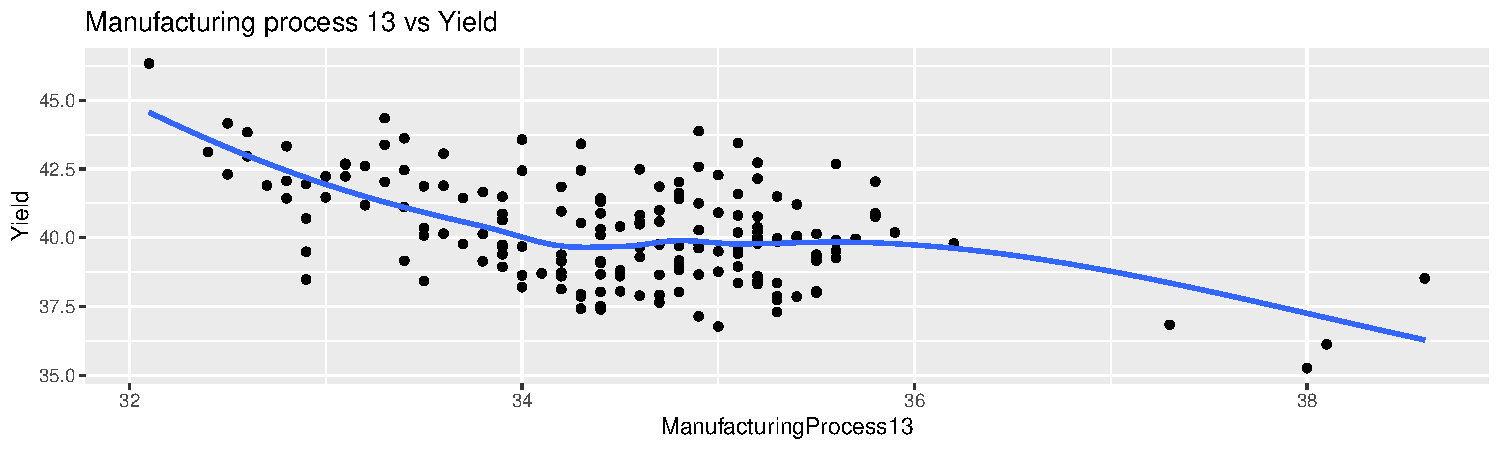
\includegraphics{Homework-Two_files/figure-latex/kj-6.3f-2.pdf}
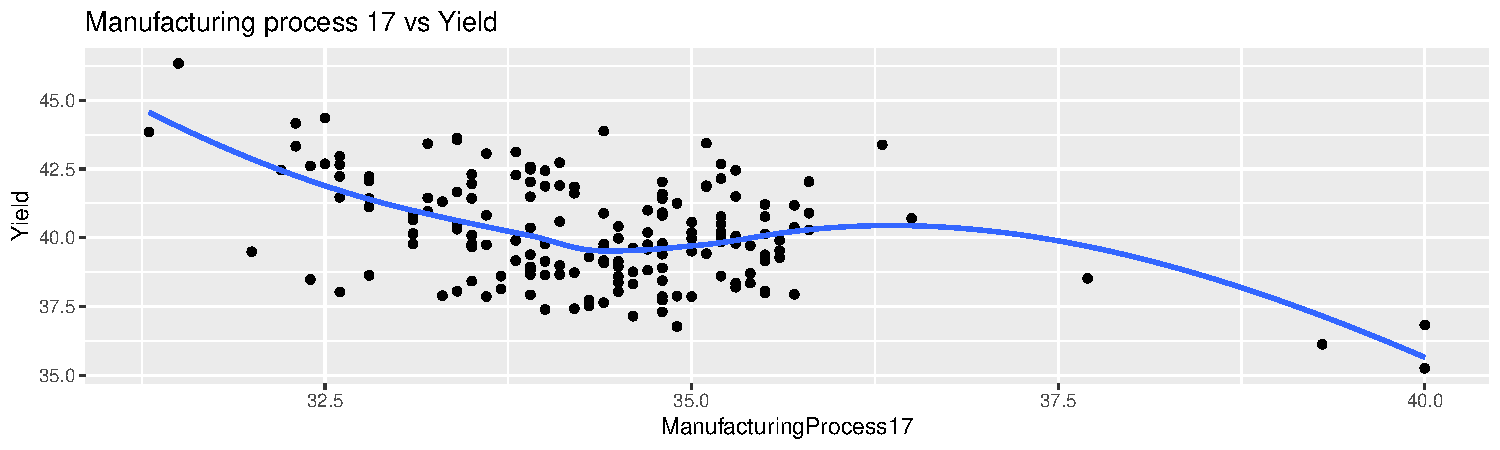
\includegraphics{Homework-Two_files/figure-latex/kj-6.3f-3.pdf}

\begin{table}[H]

\caption{\label{tab:kj-6.3f}Correlation of top 5 Important Variables vs Yield}
\centering
\begin{tabular}{l|r}
\hline
  & Yield\\
\hline
\rowcolor{gray!6}  Yield & 1.0000000\\
\hline
ManufacturingProcess32 & 0.6083321\\
\hline
\rowcolor{gray!6}  ManufacturingProcess17 & -0.4258069\\
\hline
ManufacturingProcess13 & -0.5036797\\
\hline
\rowcolor{gray!6}  ManufacturingProcess36 & -0.5013575\\
\hline
ManufacturingProcess09 & 0.5034705\\
\hline
\end{tabular}
\end{table}

Out of the top three important variables, only ManufacturingProcess32
has a positive correlation with yield. We can drill down to the extent
of the correlation with ManufacturingProcess32,ManufacturingProcess17,
and ManufacturingProcess13 vs Yield. Please note we also applied a loess
smoother in our visualizations. ManufacturingProcess13 and
ManufacturingProcess17 have a moderate negative correlation with yield,
meaning that there exists an inverse relationship between these
predictors and yield. From a business point of view, our aim is to
increase yield since we know that yield ties into revenue. We do not
have insight into what mechanics go into each manufacturing process but
we can use this knowledge to adjust the processes to emulate
manufacturing process 32.

\hypertarget{AS-2}{%
\chapter*{Assignment 2}\label{AS-2}}
\addcontentsline{toc}{chapter}{Assignment 2}

\addcontentsline{toc}{subsection}{Kuhn and Johnson 7.2}

\begin{question}{Kuhn and Johnson 7.2}Friedman (1991) introduced several benchmark data sets create by simulation. One of these simulations used the following nonlinear equation to create data: $y = 10\text{sin}(\pi x_1 x_2)+20(x_3-0.5)^2+10x_4+5x_5+N(0\text{,} \sigma^2)$; where the $x$ values are random variables uniformly distributed between $[0, 1]$ (there are also 5 other non-informative variables also created in the simulation). \end{question}

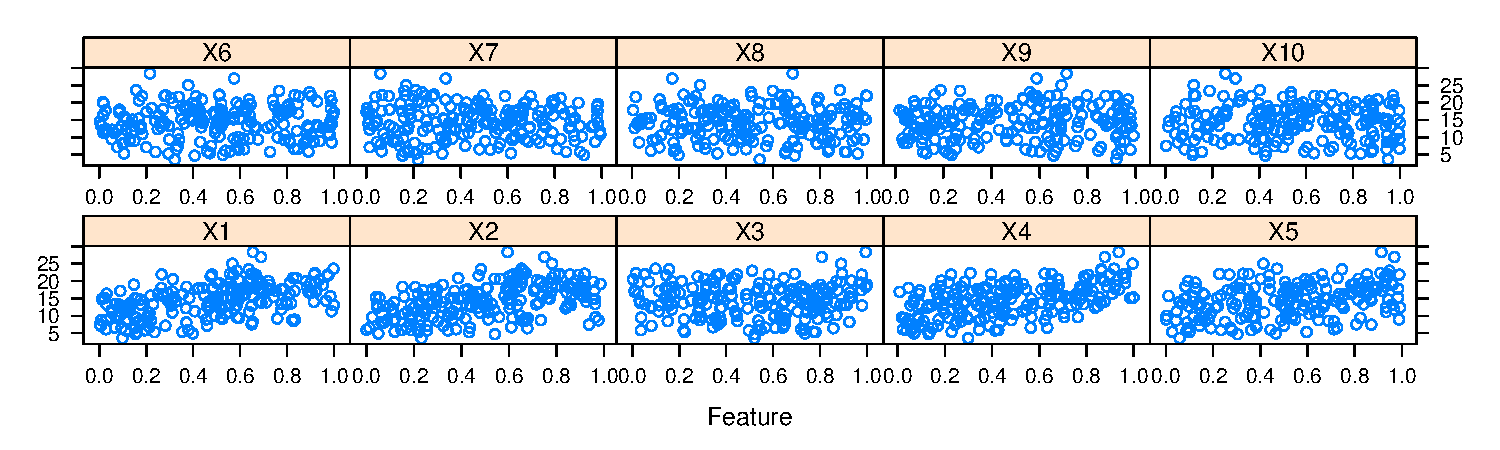
\includegraphics{Homework-Two_files/figure-latex/kj-7.2-ex1-1.pdf}

\begin{subquestion}{(a).} Tune several models on these data. For example: 
\end{subquestion}

Model 1:

Model 2:

Model 3:

\begin{subquestion}{(b).}
Which models appear to give the best performance? Does MARS select the informative predictors (those named X1-X5)?
\end{subquestion}

\addcontentsline{toc}{subsection}{Kuhn and Johnson 7.5}

\begin{question}{Kuhn and Johnson 7.5}
Exercise 6.3 describes data for a chemical manufacturing process. Use the same data imputation, data splitting, and pre-processing steps as before and train several nonlinear regression models.
\end{question}

\begin{subquestion}{(a).}
Which nonlinear regression model gives the optimal resampling and test set performance? 
\end{subquestion}

\begin{subquestion}{(b).}
Which predictors are most important in the optimal nonlinear regression model? Do either the biological or process variables dominate the list? How do the top ten important predictors compare to the top ten predictors from the optimal linear model? 
\end{subquestion}

\begin{subquestion}{(c).}
Explore the relationships between the top predictors and the response for the predictors that are unique to the optimal nonlinear regression model. Do these plots reveal intuition about the biological or process predictors and their relationship with yield?
\end{subquestion}

\hypertarget{AS-3}{%
\chapter*{Assignment 3}\label{AS-3}}
\addcontentsline{toc}{chapter}{Assignment 3}

\addcontentsline{toc}{subsection}{Kuhn and Johnson 8.1}

\begin{question}{Kuhn and Johnson 8.1} Recreate the simulated data from Exercise 7.2: \end{question}

\begin{subquestion}{(a).} Fit a random forest model to all of the predictors, then estimate the variable importance scores. Did the random forest model significantly use the uninformative predictors (V6-V10)?\end{subquestion}

\begin{subquestion}{(b).} Now add an additional predictor that is highly correlated with one of the informative predictors. Fit another random forest model to these data. Did the importance score for V1 change? What happens when you add another predictor that is also highly correlated with V1? For example:\end{subquestion}

\begin{subquestion}{(c).} Use the `cforest` function in the party package to fit a random forest model using conditional inference trees. The party package function `varimp` can calculate predictor importance. The `conditional` argument of that function toggles between the traditional importance measure and the modified version described in Strobl et al. (2007). Do these importances show the same pattern as the traditional random forest model?\end{subquestion}

\begin{subquestion}{(d).} Repeat this process with different tree models, such as boosted trees and Cubist. Does the same pattern occur?\end{subquestion}

\addcontentsline{toc}{subsection}{Kuhn and Johnson 8.2}

\begin{question}{Kuhn and Johnson 8.2}Use a simulation to show tree bias with different granularities.\end{question}

\addcontentsline{toc}{subsection}{Kuhn and Johnson 8.3}

\begin{question}{Kuhn and Johnson 8.3} In stochastic gradient boosting the bagging fraction and learning rate will govern the construction of the trees as they are guided by the gradient. Although the optimal values of these parameters should be obtained through the tuning process, it is helpful to understand how the magnitudes of these parameters affect magnitudes of variable importance. Figure 8.24 provides the variable importance plots for boosting using two extreme values for the bagging fraction (0.1 and 0.9) and the learning rate (0.1 and 0.9) for the solubility data. The left-hand plot has both parameters set to 0.1, and the right-hand plot has both set to 0.9: \end{question}

\begin{subquestion}{(a).} Why does the model on the right focus its importance on just the first few of predictors, whereas the model on the left spreads importance across more predictors? \end{subquestion}

\begin{subquestion}{(b).} Which model do you think would be more predictive of other samples?\end{subquestion}

\begin{subquestion}{(c).} How would increasing interaction depth affect the slope of predictor importance for either model in Fig.8.24?\end{subquestion}

\addcontentsline{toc}{subsection}{Kuhn and Johnson 8.7}

\begin{question}{Kuhn and Johnson 8.7}
Refer to Exercises 6.3 and 7.5 which describe a chemical manufacturing process. Use the same data imputation, data splitting, and pre-processing steps as before and train several tree-based models:
\end{question}

\begin{subquestion}{(a).} Which tree-based regression model gives the optimal resampling and test set performance? \end{subquestion}

\begin{subquestion}{(b).} Which predictors are most important in the optimal tree-based regression model? Do either the biological or process variables dominate the list? How do the top 10 important predictors compare to the top 10 predictors from the optimal linear and nonlinear models?\end{subquestion}

\begin{subquestion}{(c).} Plot the optimal single tree with the distribution of yield in the terminal nodes. Does this view of the data provide additional knowledge about the biological or process predictors and their relationship with yield?\end{subquestion}

\hypertarget{AS-4}{%
\chapter*{Assignment 4}\label{AS-4}}
\addcontentsline{toc}{chapter}{Assignment 4}

\hypertarget{tbd}{%
\section{TBD}\label{tbd}}

\hypertarget{R-Script}{%
\chapter*{R Script}\label{R-Script}}
\addcontentsline{toc}{chapter}{R Script}


\end{document}
